\documentclass[
  crop,tikz,convert={
    outext=.svg,
    command=\unexpanded{
      pdf2svg \infile\space\outfile
    }
  },
  multi=false]
{standalone}[2012/04/13]

% \usepackage{tikz}
%\usetikzlibrary{...}% tikz package already loaded by 'tikz' option above
\usetikzlibrary{positioning}

\makeatletter

\begin{document}

  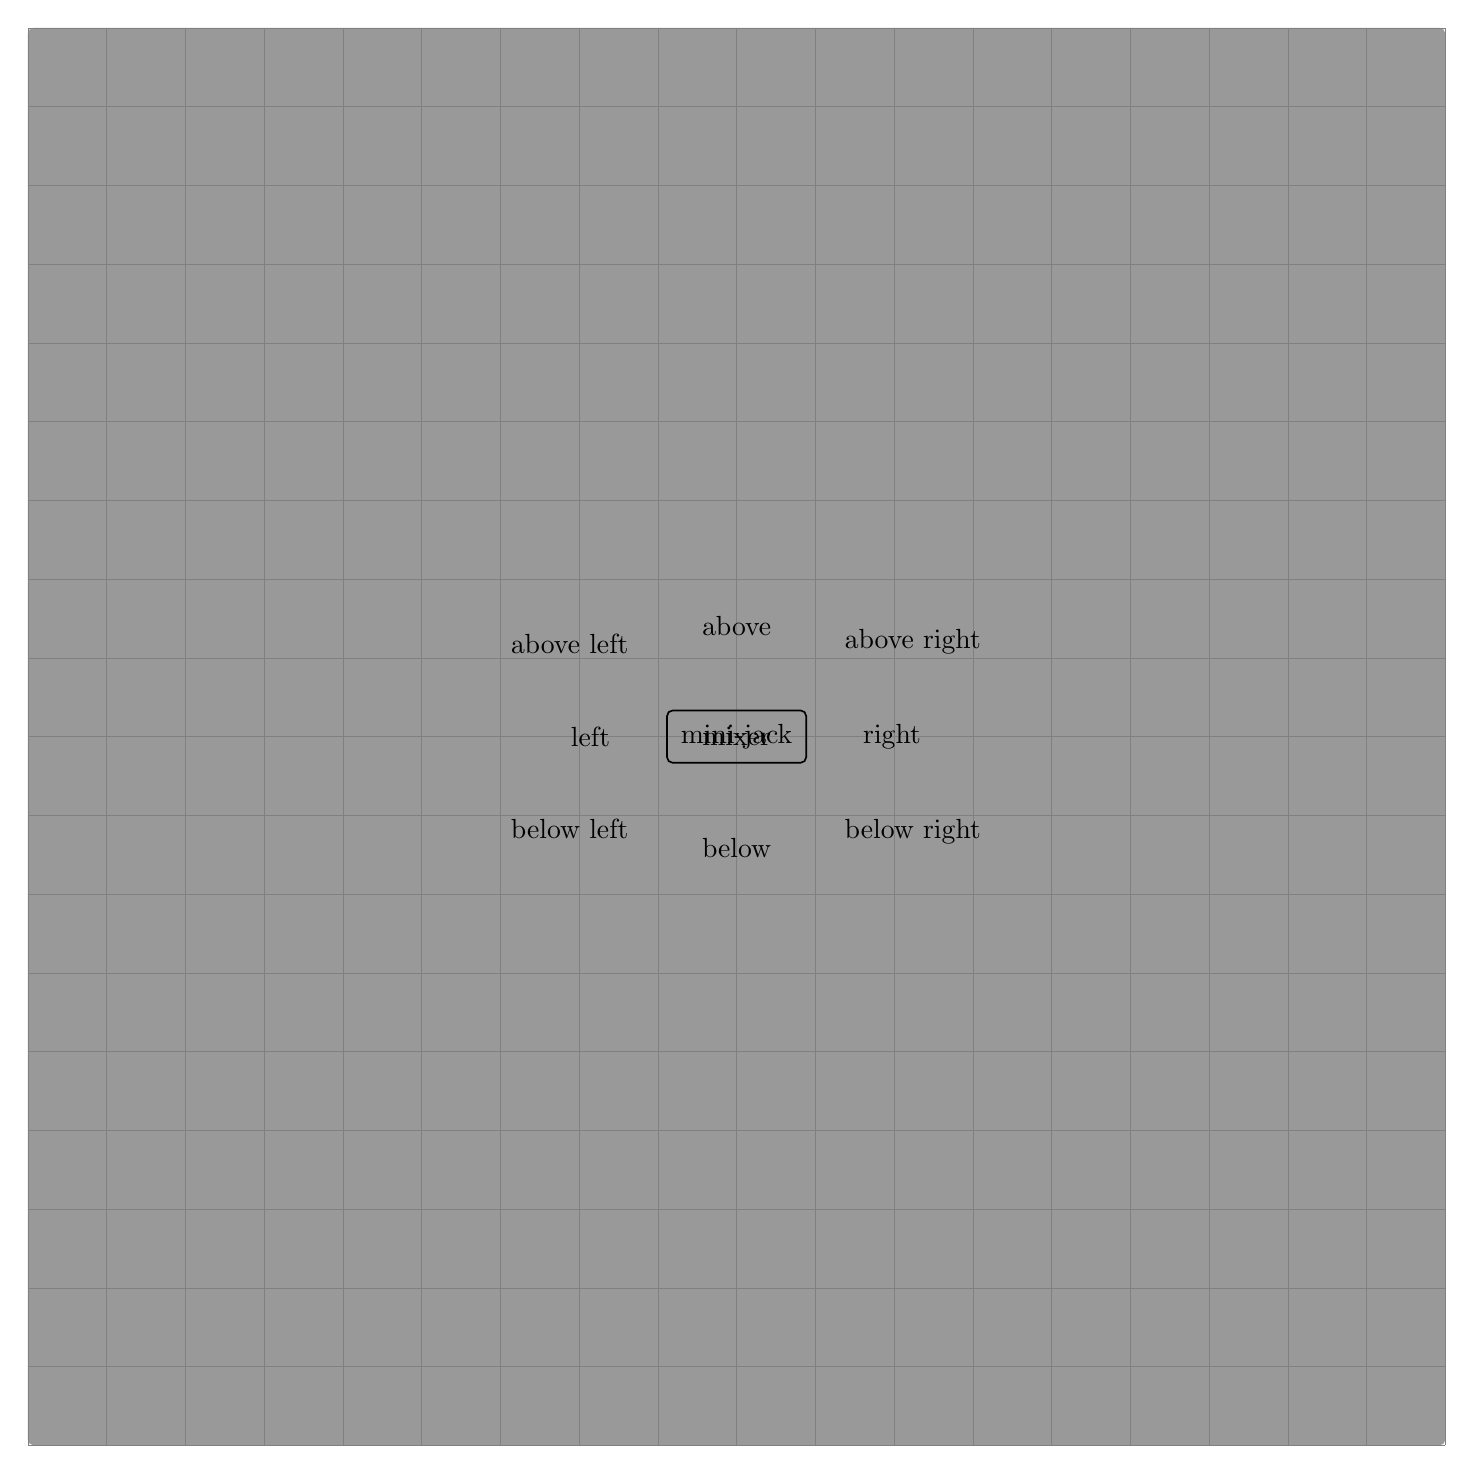
\begin{tikzpicture}[
      rounded corners=2pt,
      inner sep=5pt,
      line width=.6pt,
      node distance=.8cm]

    % background grid & fill
    % \fill[white] (0,0) rectangle (15,8);
    \fill[black!40!white] (-9,-9) rectangle (9,9);
    \draw[step=1cm,gray,very thin] (-9,-9) grid (9,9);

    \node (0) {mixer};
    \node[right=of 0] {right};
    \node[below right=of 0] {below right};
    \node[below=of 0] {below};
    \node[below left=of 0] {below left};
    \node[left=of 0] {left};
    \node[above left=of 0] {above left};
    \node[above=of 0] {above};
    \node[above right=of 0] {above right};

    % sources y=7
    \node (jack) at (0) [draw] {mini-jack};
    % \node (microphone) at (3.5,7) [draw] {microphone};
    % \node (soundcard) at (6,7) [draw] {DJ Soundcard};

    % mixer y=5
    % \node (mixer) at (3.5,5) [draw] {mixer};
    % \node (mixer) {origin} [draw] {mixer};
    % \node (headphones) at (6,5) [draw] {headphones};

    % % amps y=3
    % \node (subamp) at (2,3) [draw] {sub amp};
    % % \node (topamp) at (5,3) [draw] {top amp};

    % % speakers y=1
    % \node [draw] (subl) at (1,1) {sub-L};
    % \node [draw] (subr) at (3,1) {sub-R};
    % \node [draw] (topl) at (5,1) {top-L};
    % \node [draw] (topr) at (7,1) {top-R};

    % % wiring (sources - mixer)
    % \draw (jack.south) -- (mixer.north) node[midway,above] {$C_1$};
    % \draw (microphone.south) -- (mixer.north) node[midway,above] {$C_2$};
    % \draw (soundcard.south) -- (mixer.north) node[midway,above] {$C_3$};
    % \draw (soundcard.south) -- (headphones.north) node[midway,above] {$C_4$};

    % % wiring (amps - speakers)
    % \draw (mixer.south) -- (topl.north) node[midway,above] {$C_5$};
    % \draw (mixer.south) -- (topr.north) node[midway,above] {$C_5$};
    % \draw (mixer.south) -- (subamp.north) node[midway,above] {$C_6$};

    % % wiring (amps - speakers)
    % \draw (subamp.south) -- (subl.north) node[midway,above] {$C_7$};
    % \draw (subamp.south) -- (subr.north) node[midway,above] {$C_7$};

    % % cable legend
    % \node (legend) at (11,4) [draw, text width=6cm] {
    %   \textbf{Cables} (top to bottom)\\
    %   $C_1$ - stereo-mini-jack - 2xRCA\\
    %   $C_2$ - mhicrophone - mono jack\\
    %   $C_3$ - 2xRCA - 2xRCA\\
    %   $C_4$ - stereo-jack - headphones\\
    %   $C_5$ - speakON - speakON\\
    %   $C_6$ - mono jack - mono jack\\
    %   $C_7$ - speakON - XLR\\
    % };

  \end{tikzpicture}
\end{document}
